%++++++++++++++++++++++++++++++++++++++++
% Don't modify this section unless you know what you're doing!
\documentclass[a4paper,14pt]{article}
\usepackage{listings} % code blocks
\usepackage{tabularx} % extra features for tabular environment
\usepackage{amsmath}  % improve math presentation
\usepackage{graphicx} % takes care of graphic including machinery
\usepackage{subcaption} % necessary for subfigures
\usepackage[margin=2cm,a4paper,nohead]{geometry} % decreases margins
\usepackage{cite} % takes care of citations
\usepackage[final]{hyperref} % adds hyper links inside the generated pdf file

%++++++++++++++++++++++++++++++++++++++++


\begin{document}

\title{Exercise 2: LeNet in Tensorflow}
\author{David-Elias K\"unstle}
\date{\today}
\pagenumbering{gobble} % turn of page numbering (not needed for 2 pages)
\maketitle
\section{Introduction}

In this report I present two small experiments on handwritten digit detection
(\emph{MNIST dataset}) with a LeNet-like convolutional neural network.
The network consists of two convolutional layers with 16 3x3 filters (stride 1, same
padding), both with ReLu activation and max pooling,
followed by a fully connected layer with 128 hidden units and 10 output units
after a softmax.
It is implemented in \emph{python3} using the \emph{Tensorflow library}
(\texttt{tensorflow-gpu 1.3.0}).
For training 50.000 digit-label pairs were used. The validation set contains
10.000 ones which are not in the training set.


\section{Changing the Learning Rate}

The influence of learning rate on validation error is what we see in
\autoref{fig:error}.
You see the lower error rate while all epochs the higher the learning
rate ($\alpha$) is.

For $\alpha \in \{0.001, 0.01, 0.1\}$ error rate drops in the first 1--4 epochs
and converges afterwards.
Still the steepness while the drop and the value of the limit differ depending
on $\alpha$.
I assume, that the error rates after training will stay almost constant, even if we
would add some epochs.
Instead the course for $\alpha = 0.0001$ is looks like linear
decrease.
It's highly likely that while additional training epochs the error rate could decrease further
and start converging later.

I would prefer $\alpha=0.1$ because it converges quickly to the lowest error rate.
Training could be stopped after just one or two epochs.
Nonetheless we know, that high learning rates increase the risk for overshooting
and other problems while training.

\begin{figure}[ht]
  \centering 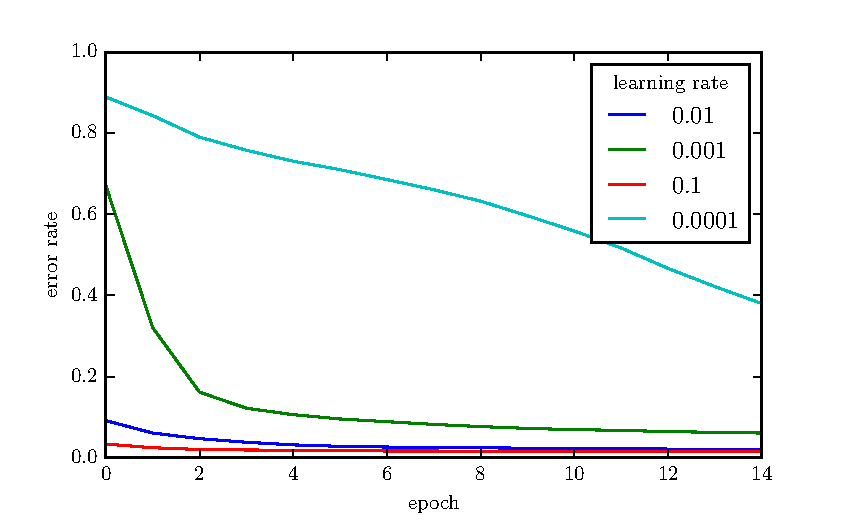
\includegraphics[width=0.9\textwidth]{assets/error.pdf}
  \caption{
    \label{fig:error}
    Error rate on validation dataset of LeNet-like CNN while ongoing training
    with various learning rates.
  }
\end{figure}

\section{Runtime on CPU vs GPU}

Each value of the filters in a convolutional layer is a parameter learned while training.
A convolutional layer in our network therefore has
$\texttt{input dimension} \times \texttt{filter width} \times \texttt{filter
  height} \times \texttt{number filters}$ parameters.
Our LeNet-like network with 16 filters per convolutional layer has
about 5.000 parameters in the convolutional layers and about 3.500 ones in the
fully connected parts.
By exponential increase in the number of filters we
exponentially increase the number of parameters
and therefore the training complexity.
The dominance of parameters in the convolutional layers versus the fully
connected layer increases dramatically.

While experimenting with various filter sizes I had especially problem with
the limited memory size on GPU.
While prediction e.g. for classification error calculation,
the full MNIST training dataset got processed.
3GB gRAM was too small for the high dimensional output of convolution layers
with high number of filter.
As a workaround I modified the code to always process batches of the dataset.

In \autoref{fig:runtime} you'll see how different number of filters affects the
training time on CPU and GPU.
The CPU is always slower than the GPU.
We expect this because the GPU is optimized for matrix operations and parallel
executions. This is handy for forward and backpropagation of our network.
For the exponential increase in filter number the CPU runtime
increases also exponential-like.
The CPU has to process the operations sequentially wherefore double the time is necessary
for double the parameters.
On GPU runtime just slightly increases by increasing filter number up to $2^5$.
The GPU can compensate the increase of parameters by massive parallel
processing. Still, for higher filter numbers all parallel processing units are
in use such that the additional ones have to be processed in sequence as well.
Therefore runtime ascends quickly for higher number of filters.

\begin{figure}[ht]
  \centering 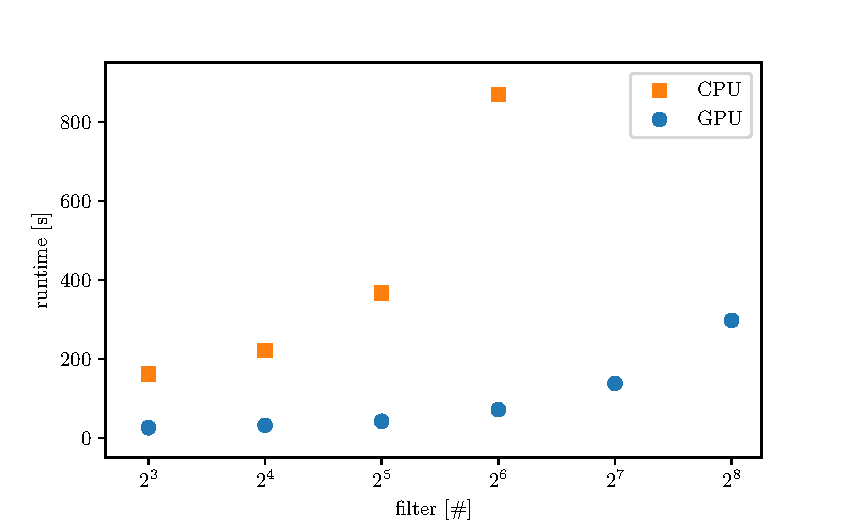
\includegraphics[width=0.9\textwidth]{assets/runtime.pdf}
  \caption{
    \label{fig:runtime} Runtime for 10 training epochs with LeNet-like CNN and MNIST
    dataset on GPU and CPU.
    The number of filters per convolutional layer was modulated.
    The code was executed on a workstation
    with \emph{Intel\textregistered Core\texttrademark i7-3770 CPU @ 3.40GHz} and
    \emph{NVIDIA GeForce GTX 1060}.
  }
\end{figure}


% \begin{thebibliography}{99}
% \end{thebibliography}

\end{document}
